\documentclass[11pt, oneside]{article}   	% use "amsart" instead of "article" for AMSLaTeX format
\usepackage{geometry}                		% See geometry.pdf to learn the layout options. There are lots.
\geometry{letterpaper}                   		% ... or a4paper or a5paper or ... 
%\geometry{landscape}                		% Activate for rotated page geometry
%\usepackage[parfill]{parskip}    		% Activate to begin paragraphs with an empty line rather than an indent
\usepackage{graphicx}				% Use pdf, png, jpg, or eps§ with pdflatex; use eps in DVI mode
								% TeX will automatically convert eps --> pdf in pdflatex		
\usepackage{amssymb,amsmath}
\usepackage{float}

\usepackage{listings}
\usepackage[utf8]{inputenc}
\newcommand{\Var}{\operatorname{Var}}
\newcommand{\E}{\operatorname{E}}
\newcommand{\Cov}{\operatorname{Cov}}
% Default fixed font does not support bold face
\DeclareFixedFont{\ttb}{T1}{txtt}{bx}{n}{12} % for bold
\DeclareFixedFont{\ttm}{T1}{txtt}{m}{n}{12}  % for normal

\lstset{language=R,
    basicstyle=\small\ttfamily,
    stringstyle=\color{DarkGreen},
    otherkeywords={0,1,2,3,4,5,6,7,8,9},
    morekeywords={TRUE,FALSE},
    deletekeywords={data,frame,length,as,character},
    keywordstyle=\color{blue},
    commentstyle=\color{DarkGreen},
     %frame=single, % adds a frame around the code
     backgroundcolor=\color{lightgray},
}
\usepackage[svgnames]{xcolor}
\title{STAT211 Mandatory Homework 2}
\author{Yapi Donatien Achou}
%\date{}							% Activate to display a given date or no date

\begin{document}
\maketitle

\section{Problem 2.1}
let  $X_{t}$ be given by 
\begin{equation}
X_{t} = \beta_{0} + \beta_{1}t + Z_{t}
\end{equation}
where $Z_{t}$ is an independent random variable with mean 0 and variance $\sigma^{2}$.
\subsection{Part A: Prove that $X_{t}$ is non stationary}
\begin{equation}
\begin{aligned}
\mu_{X}(t)  &= E[X_{t}]\\
&=E[\beta_{0} + \beta_{1}t + Z_{t}]\\
&=E[\beta_{0}] + E[\beta_{1}t] + E[Z_{t}]\\
&=\beta_{0} + \beta_{1}t
\end{aligned}
\end{equation}
Since $\mu_{X}(t) $ depends on $t$, we conclude that $X_{t}$ is non-stationary.

\subsection{Part b}
let $\Delta X$ be given by 
\begin{equation}
\Delta X = X_{t} - X_{t-1} = \beta_{1} + Z_{t} - Z_{t-1}
\end{equation}
Then 
\begin{equation}
\begin{aligned}
E[\Delta X] &= E[\beta_{1} + Z_{t} - Z_{t-1}]\\
&=E[\beta_{1}]+E[Z_{t}] -E[Z_{t-1}] \\
&=\beta_{1}
\end{aligned}
\end{equation}

\begin{equation}
\begin{aligned}
\gamma_{X}(t+h,t) &= \Cov(\beta_{1} + Z_{t+h} - Z_{t+h-1},\beta_{1} + Z_{t} - Z_{t-1})\\
&=\Cov( Z_{t+h} - Z_{t+h-1}, Z_{t} - Z_{t-1})\\
&= \Cov( Z_{t+h},Z_{t}) - \Cov( Z_{t+h},Z_{t-1}) -\Cov( Z_{t+h-1},Z_{t}) +\Cov( Z_{t+h-1},Z_{t-1}) \\
&=\sigma_{z}^{2}( \delta_{h,0} - \delta_{h,-1} - \delta_{h,1} + \delta_{h,0})\\
& = 
     \begin{cases}
       2\sigma_{z}^{2} &\quad\text{if h=0}\\
       -\sigma_{z}^{2}&\quad\text{if h = $\pm$ 1} \\
       0 &\quad\text{otherwise}
     \end{cases}
\end{aligned}
\end{equation}
$E[\Delta X]$ and $\gamma_{X}(t+h,t)$ are independent of $t$, therefore $\Delta X$ is stationary

\section{Part c}
If $Z_{t}$ is replaced by a general process $Y_{t}$ with mean $\mu_{Y}$ and auto-covariance function $\gamma_{Y}(h)$.
\begin{equation}
\begin{aligned}
E[\Delta X] &= E[\beta_{1} + Y_{t} - Y_{t-1}]\\
&=E[\beta_{1}]+E[Y_{t}] -E[Y_{t-1}] \\
&=\beta_{1}+\mu_{Y} -\mu_{Y} \\
&=\beta_{1}
\end{aligned}
\end{equation}
The mean is independent of $t$. For the auto-covariance function we use the same computation as in question b.








%%%%%%%%%%%%%%%%%%%%%%%%%%%%%%%%%%%%%%%%%%%%%%%%%%%%%%%%%%%%%%%%%%%%%%%%%%%%%%%%%%%%
%%%%%%%%%%%%%%%%%%%%%%%%%%%%%%%%%%%%%%%%%%%%%%%%%%%%%%%%%%%%%%%%%%%%%%%%%%%%%%%%%%%%
%%%%%%%%%%%%%%%%%%%%%%%%%%%%%%%%%%%%%%%%%%%%%%%%%%%%%%%%%%%%%%%%%%%%%%%%%%%%%%%%%%%%
%%%%%%%%%%%%%%%%%%%%%%%%%%%%%%%%%%%%%%%%%%%%%%%%%%%%%%%%%%%%%%%%%%%%%%%%%%%%%%%%%%%%

\section{Problem 2.2}
\subsection{Introduction}
In this section we analyse the varve glacial data and perform different statistical transformation of the data. A varve is an annual layer of sediment [wikipedia]
\subsection{Part a). Plot}
\begin{figure}[H] %  figure placement: here, top, bottom, or page
   \centering
   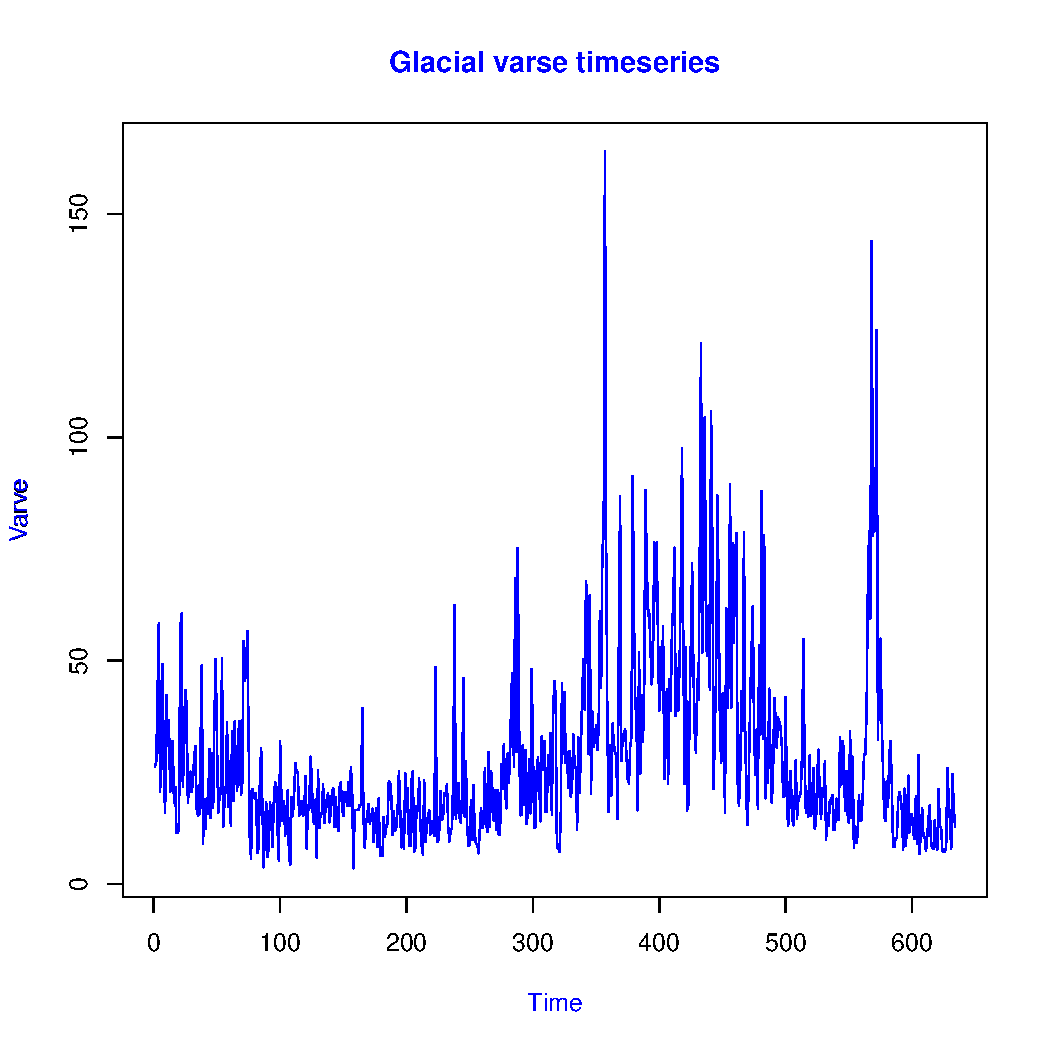
\includegraphics[width=4in]{sample_plot} 
   \caption{Plot of the glacial varve data}
   \label{fig:varve}
\end{figure}
From Figure \ref{fig:varve} we see that the varve glacial data exhibits some nonstationarity. To improve the nonstationarity we can use a logarithmic and a differencing transformation.
%%%%%%%%%%%%%%%%%%%%%%%%%%%%%%%%%%%%%%%%%%%%%%%%%%%%%%%%%%%%%%%%%%%%%%%%%%%%%%%%%%%%
%%%%%%%%%%%%%%%%%%%%%%%%%%%%%%%%%%%%%%%%%%%%%%%%%%%%%%%%%%%%%%%%%%%%%%%%%%%%%%%%%%%%
\subsection{Part b). Heteroscedasticity of the varve data}
A collection of random variables is heteroscedastic if there are sub-population that have different variability, where the variability can be measured by any statistical dispersion [wikipedia]. We use the variance to show that the varve data exhibits some Heteroscedasticity by computing and comparing the variance of the first and the second half of the data. 
\begin{flushleft}
Let $X_{t}$ be the varve time series. The R code bellow computes the variance of the first and second half of $X_{t}$.
\end{flushleft}
\clearpage
\begin{lstlisting}
library(astsa)
data(varve)

index <- length(varve)/2
variance_first_half <- var(varve[0:index])
variance_second_half <- var(varve[index:length(varve)])

print(variance_first_half)
>>  133.4574
print(variance_second_half)
>>  592.9645
\end{lstlisting}
\begin{flushleft}
We see that the variance of the second half of the data is approximately \textcolor{blue}{4.44} time larger than the variance of the first half of the data. This shows that the first and the second half of the data have significantly different variability. Therefore the time series $X_{t}$ exhibits Heteroscedasticity.
\end{flushleft}

\begin{flushleft}
Now, let $Y_{t}$ be the log transformation of $X_{t}$
\begin{equation}
Y_{t} = \log(X_{t})
\end{equation}
\end{flushleft}

\begin{lstlisting}
library(astsa)
data(varve)

index <- length(varve)/2
variance_loga_first_half <- var(log(varve[0:index]))
variance_loga_second_half <- var(log(varve[index:length(varve)]))

print(variance_loga_first_half)
>>  0.2707217
print(variance_loga_second_half)
>>  0.4506843
\end{lstlisting}
\begin{flushleft}
We can observe that after the log transformation the variance of the second half of $Y_{t}$ is \textcolor{blue}{1.66} time larger than the the first half. This shows that the heteroscedasticity has been significantly reduced.
\end{flushleft}
\begin{figure}[H] %  figure placement: here, top, bottom, or page
   \centering
   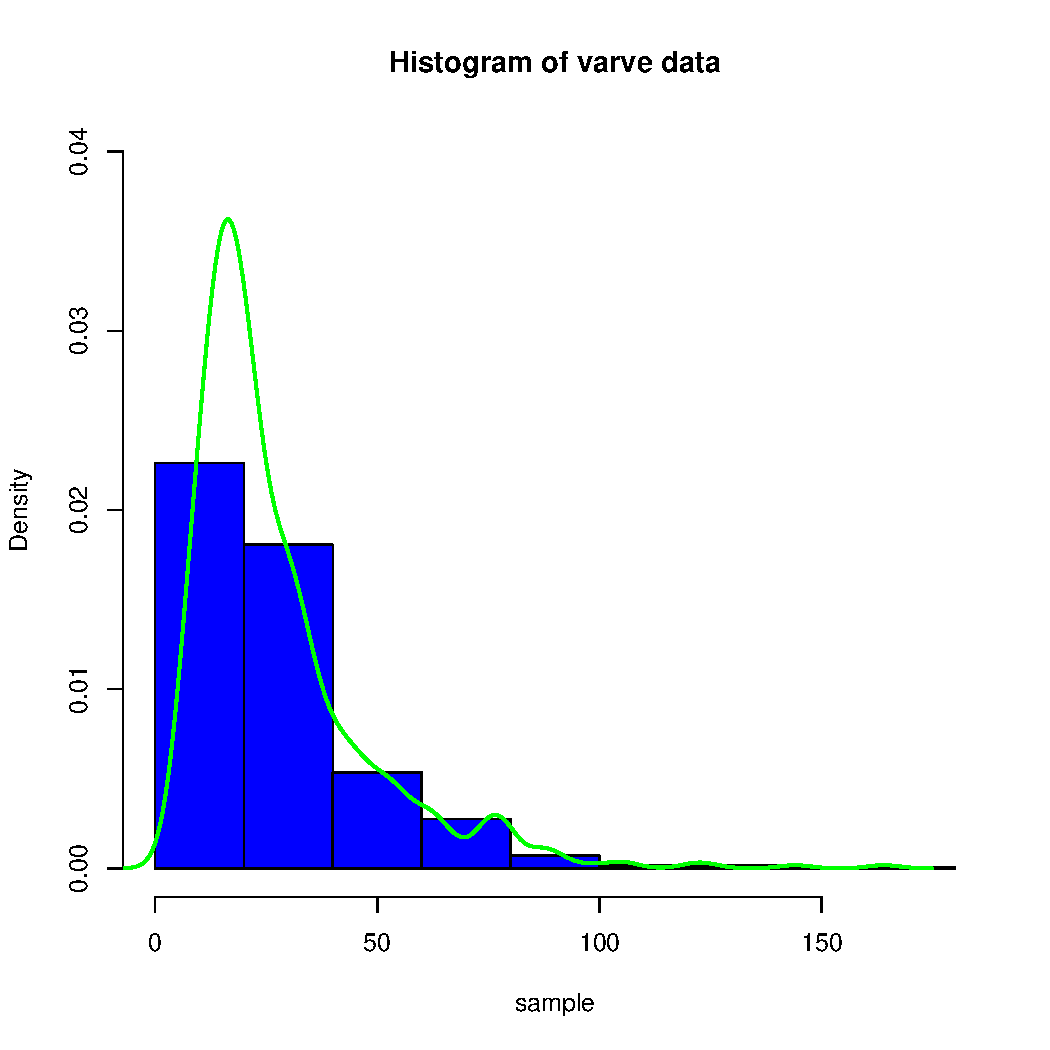
\includegraphics[width=2.5in]{hist_x} 
   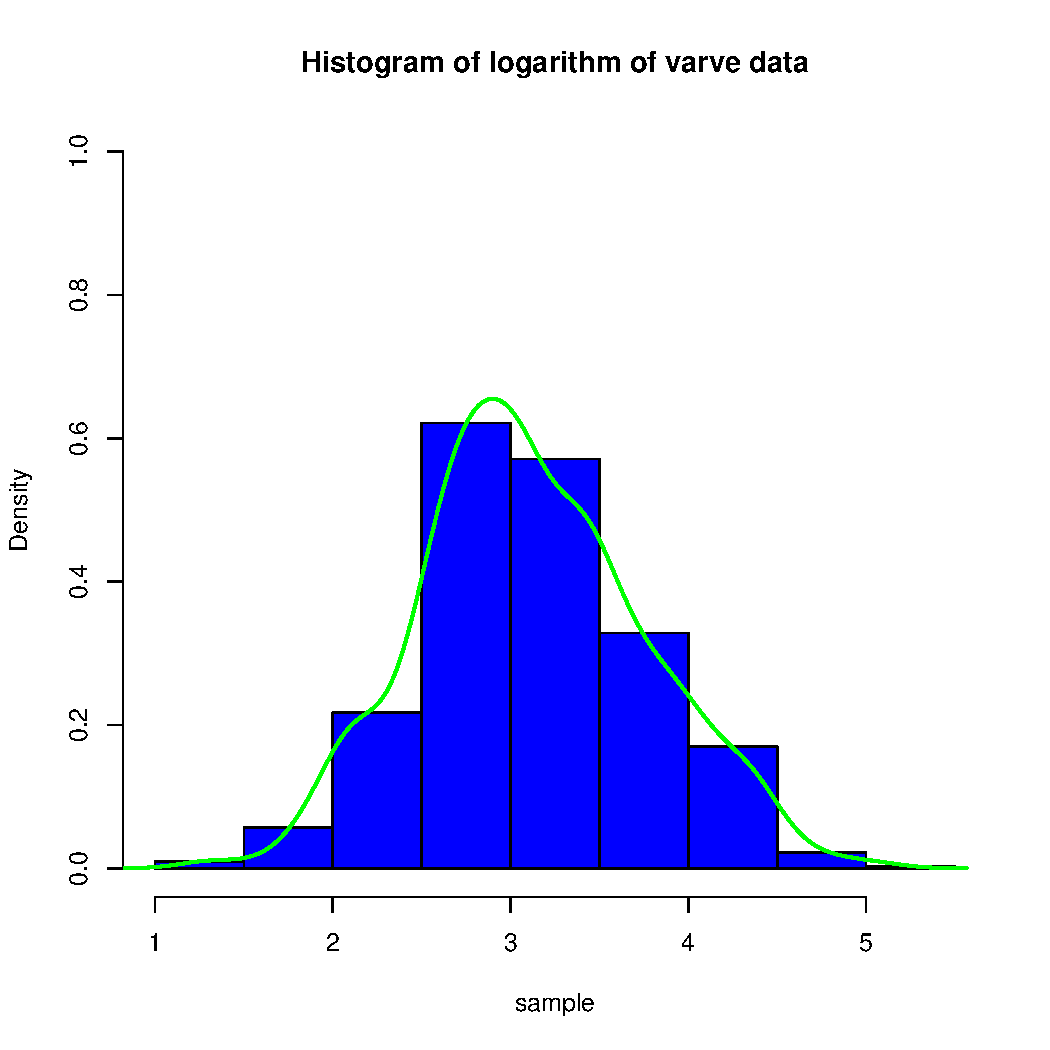
\includegraphics[width=2.5in]{hist_log}
   \caption{Histogram of varve data (left) and histogram of the log transformation of varve data (right)}
   \label{fig:hist}
\end{figure}
From Figure \ref{fig:hist} we see that the histogram of the varve data $X_{t}$ is skewed to the right, but the log transformation $Y_{t} = \log(X_{t})$ is approximately normally distributed.

\subsection{Part c). Plot of $Y_{t}$}
\begin{figure}[H] %  figure placement: here, top, bottom, or page
   \centering
   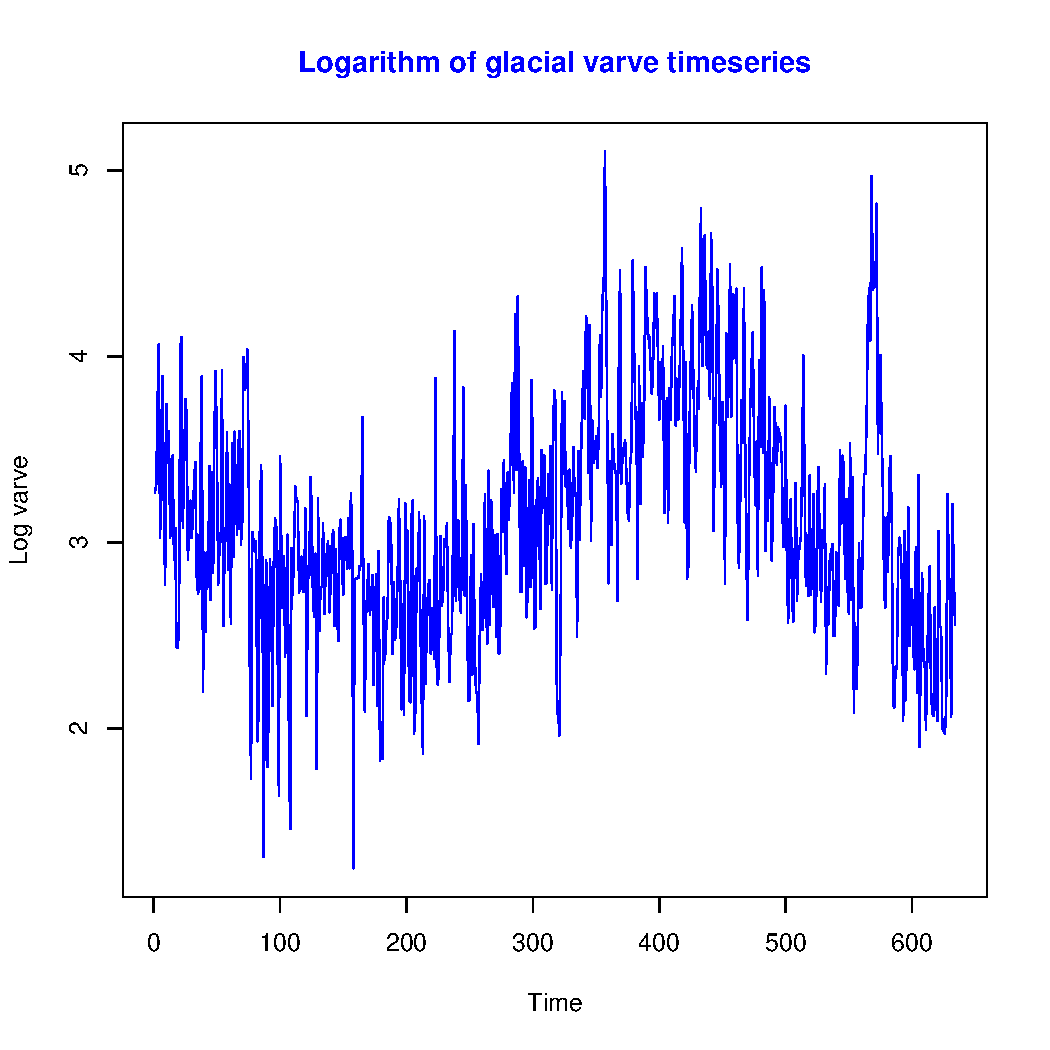
\includegraphics[width=4in]{var_sample_plot} 
   \caption{example caption}
   \label{fig:example}
\end{figure}

%%%%%%%%%%%%%%%%%%%%%%%%%%%%%%%%%%%%%%%%%%%%%%%%%%%%%%%%%%%%%%%%%%%%%%%%%%%%%%%%%%%%
%%%%%%%%%%%%%%%%%%%%%%%%%%%%%%%%%%%%%%%%%%%%%%%%%%%%%%%%%%%%%%%%%%%%%%%%%%%%%%%%%%%%
\subsection{Part d). Sample Auto covariance Function of $Y_{t}$}
\begin{figure}[H] %  figure placement: here, top, bottom, or page
   \centering
   
\includegraphics[width=4in]{acf} 
   \caption{Sample Autocorrelation Function (ACF) of $Y_{t}$ the log of the varve data and the bound $\pm 1.96\sqrt{n}$ (the dash blue line)}
   \label{fig:acf}
\end{figure}
From Figure \ref{fig:acf}, we see that the sample ACF of $Y_{t}$ is a decreasing function of lag with local maximum. We also observe some periodicity. Since the sample correlation function of $Y_{t}$ is slowly decaying with some period, this suggests some trend and seasonality.
%We also observe that all the ACF values fall outside of the upper bound $95\%$ confidence interval $1.96\sqrt{n}$, where $n$ is the sample size.

%%%%%%%%%%%%%%%%%%%%%%%%%%%%%%%%%%%%%%%%%%%%%%%%%%%%%%%%%%%%%%%%%%%%%%%%%%%%%%%%%%%%
%%%%%%%%%%%%%%%%%%%%%%%%%%%%%%%%%%%%%%%%%%%%%%%%%%%%%%%%%%%%%%%%%%%%%%%%%%%%%%%%%%%%

\section{Part e): Compute the difference $U_{t} = Y_{t}-Y_{t-1}$}
let $U_{t}$ be the difference
\begin{equation}\label{eq:diff}
U_{t} = Y_{t}-Y_{t-1} = \log(X_{t}) - \log(X_{t-1})
\end{equation}
where $X_{t}$ is the varve glacial time series.

\begin{figure}[H] %  figure placement: here, top, bottom, or page
   \centering
   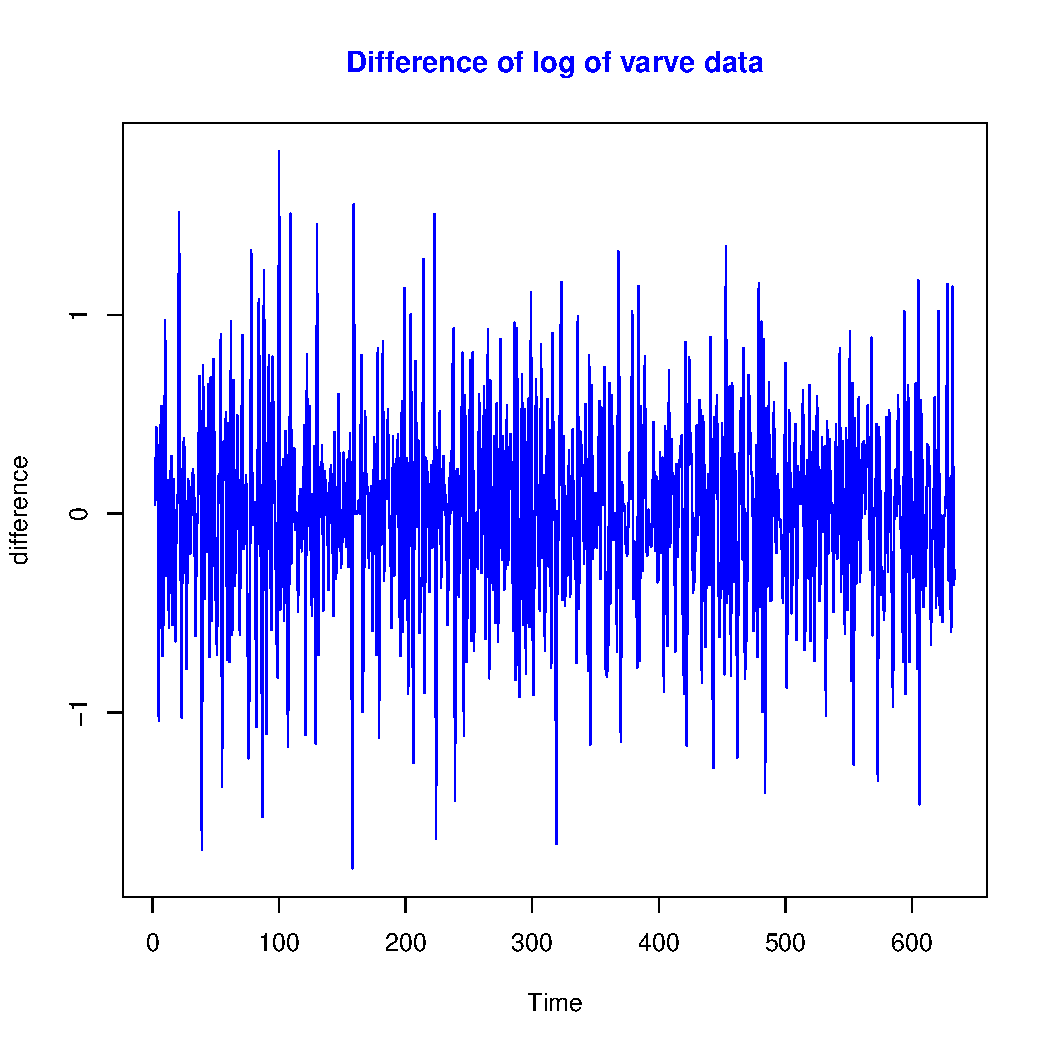
\includegraphics[width=2.5in]{diff} 
    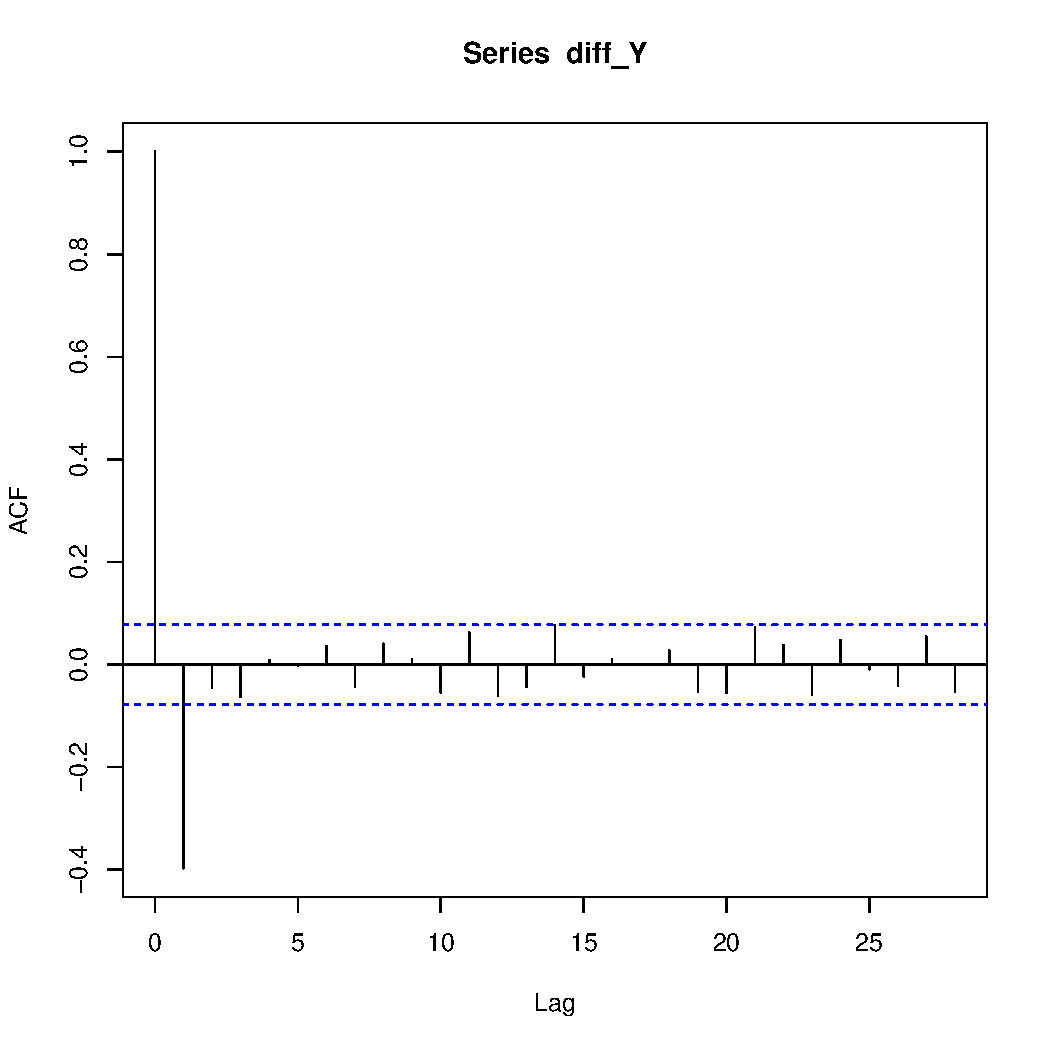
\includegraphics[width=2.5in]{acf_diff_Y} 
   \caption{Plot of the first order difference $U_{t}=Y_{t}-Y_{t-1}$ (left) and its sample Autocorrelation Function (right)}
   \label{fig:diff_acf}
\end{figure}
\begin{flushleft}
From Figure \ref{fig:diff_acf}, we observe that the sample correlation function (right plot) does not exhibits any upwards or downwards trend, showing that the mean is independent of $t$. There is also no seasonality, suggesting that the variance is the same for all $t$. Most of the values fall within the bound $\pm1.96\sqrt{n}$. The correlation at any lag is significantly closer to 0, suggesting that $U_{t+h}$ and $U_{t}$ are independent. This suggests that the sample correlation function $\gamma_{U}$ is independent of $t$. Therefore, the differencing 
defined in equation (\ref{eq:diff}) produces a reasonably stationary time series.
\end{flushleft}
\begin{flushleft}
The differencing defined in equation  (\ref{eq:diff}) can be practically interpreted as a trend remover or trend eliminator.
\end{flushleft}
%%%%%%%%%%%%%%%%%%%%%%%%%%%%%%%%%%%%%%%%%%%%%%%%%%%%%%%%%%%%%%%%%%%%%%%%%%%%%%%%%%%%
%%%%%%%%%%%%%%%%%%%%%%%%%%%%%%%%%%%%%%%%%%%%%%%%%%%%%%%%%%%%%%%%%%%%%%%%%%%%%%%%%%%%
\section{Part f)}
Let $U_{t}$ be modelled by the process 
\begin{equation}\label{eq:e}
U_{t} = \mu + Z_{t} + \theta Z_{t-1}
\end{equation}
This process belonged to the following class of stationary process:
\begin{equation}\label{eq:sp}
X_{t} = \mu + \sum_{j=-\infty}^{\infty}\psi_{j}Z_{t-j}
\end{equation}
where 
\begin{equation}
\{ Z_{t} \} \sim WN(0,\sigma_{z}^{2})
\end{equation}
and 
\begin{equation}
\sum_{j=-\infty}^{\infty}|\psi_{j}| < \infty.
\end{equation}
By comparing (\ref{eq:e}) and (\ref{eq:sp}) we see that $\psi_{0} = 1$ and   $\psi_{1} = \theta$. Since $U_{t}$ is reasonably approximated a stationary time series it can be modelled by (\ref{eq:e}).
\begin{flushleft}
Now let compute $\gamma_{u}(t+h,t)$ for $U_{t}$ given by equation (\ref{eq:e}).
\end{flushleft}

\begin{equation}
\begin{aligned}
\gamma_{u}(t+h,t) &= \Cov(U_{t+h},U_{t})\\ \nonumber
 &= \Cov(\mu + Z_{t+h} + \theta Z_{t+h-1},\mu + Z_{t} + \theta Z_{t-1})\\
 &=\Cov(Z_{t+h} + \theta Z_{t+h-1}, Z_{t} + \theta Z_{t-1}) \\
 &=\Cov(Z_{t+h},Z_{t})+\theta\Cov(Z_{t+h}, Z_{t-1})+\theta\Cov(Z_{t+h-1},Z_{t}) + \theta^{2}\Cov(Z_{t+h-1},Z_{t-t})\\
 &=\sigma_{z}^{2}\delta_{h,0}+\theta\sigma_{z}^{2}\delta_{h,-1}+\theta\sigma_{z}^{2}\delta_{h,1}+\theta^{2}\sigma_{z}^{2}\delta_{h,0}\\
 &=\sigma_{z}^{2}(\delta_{h,0}+\theta\delta_{h,-1}+\theta\delta_{h,1}+\theta^{2}\delta_{h,0}  )
\end{aligned}
\end{equation}


\begin{itemize}
\item if h = 0, then
\begin{equation}
\begin{aligned}
\gamma_{u}(t+h,t) &= \sigma_{z}^{2}(\delta_{0,0}+\theta\delta_{0,-1}+\theta\delta_{0,1}+\theta^{2}\delta_{0,0}  )\\
 &=\sigma_{z}^{2}(1+0\theta+0\theta+1\theta^{2} )\\
 &=\sigma_{z}^{2}(1+\theta^{2} )
 \end{aligned}
 \end{equation}
 
 \item if h = 1, then
\begin{equation}
\begin{aligned}
\gamma_{u}(t+h,t) &= \sigma_{z}^{2}(\delta_{1,0}+\theta\delta_{1,-1}+\theta\delta_{1,1}+\theta^{2}\delta_{1,0}  )\\
 &=\sigma_{z}^{2}(0+ 0\theta+1\theta+0\theta^{2} )\\
 &=\sigma_{z}^{2}\theta
 \end{aligned}
 \end{equation}
 
  \item if h = -1, then
\begin{equation}
\begin{aligned}
 \gamma_{u}(h) &= \sigma_{z}^{2}(\delta_{-1,0}+\theta\delta_{-1,-1}+\theta\delta_{-1,1}+\theta^{2}\delta_{-1,0}  )\\
 &=\sigma_{z}^{2}(0+ 1\theta+0\theta+0\theta^{2} )\\
 &=\sigma_{z}^{2}\theta
 \end{aligned}
 \end{equation}
 
  \item if h = a, where $a \neq \pm 1$ and $a \neq 0$
\begin{equation}
\begin{aligned}
\gamma_{u}(t+h,t)&= \sigma_{z}^{2}(\delta_{a,0}+\theta\delta_{a,-1}+\theta\delta_{a,1}+\theta^{2}\delta_{a,0}  )\\
 &=\sigma_{z}^{2}(0+ 0\theta+0\theta+0\theta^{2} )\\
 &=0
 \end{aligned}
 \end{equation}
\end{itemize}

Therefore 
\[   
\gamma_{u}(t+h,t)= 
     \begin{cases}
       \sigma_{z}^{2}(1+\theta^{2} ) &\quad\text{if h=0}\\
       \theta \sigma_{z}^{2}&\quad\text{if h = $\pm$ 1} \\
       0 &\quad\text{otherwise}
     \end{cases}
\]

\section{Part g}
\begin{equation}
\hat{\rho}_{u}(1) = \frac{\hat{\gamma}_{u}(1)}{\hat{\gamma}_{u}(0)} = \frac{\theta}{1+\theta^{2}}
\end{equation}

From R code we have 
\begin{lstlisting}
library(astsa)
data(varve)
Y <- log(varve)
U <- diff(Y,lag=1, differences=1)
emp_auto_corr_rho <- acf(U,type = "correlation")
emp_auo_variance_gamma <- acf(U, type = "covariance")
print(emp_auto_corr_rho[1])

>> -0.397
\end{lstlisting}
We have 
\begin{equation}
\hat{\rho}_{u}(1) = \frac{\hat{\gamma}_{u}(1)}{\hat{\gamma}_{u}(0)} = \frac{\theta}{1+\theta^{2}} = -0.397
\end{equation}
From which we get 
\begin{equation}
0.397 + \theta + 0.397\theta^{2}  = 0
\end{equation}
with 
\begin{equation}
 \theta_{1} \approx -0.49\quad \theta_{2} \approx -2
\end{equation}

Now 
\begin{equation}
\begin{aligned}
\Var(U) &= \Cov(U,U) \\
&=\Cov(\mu + Z_{t} + \theta Z_{t-1}, \mu + Z_{t} + \theta Z_{t-1})\\
&=\Cov( Z_{t}, Z_{t})+\theta\Cov( Z_{t}, Z_{t-1})+\theta\Cov( Z_{t-1}, Z_{t})+\theta^{2}\Cov( Z_{t-1}, Z_{t-1})\\
&=\sigma_{z}^{2}(1+2\theta+\theta^{2})
\end{aligned}
\end{equation}
From the data the sample variance is 
\begin{lstlisting}
library(astsa)
data(varve)
Y <- log(varve)
U <- diff(Y,lag=1, differences=1)
variance_U <- var(U)
print(variance_U)
>> 0.3322131
\end{lstlisting}
and 
\begin{equation}
\sigma_{z}^{2} = \frac{\Var(U)}{(1+2\theta+\theta^{2})} 
\end{equation}
from which we get
\begin{equation}
 \sigma_{z}^{2} \approx 1.32726\quad or \quad  \sigma_{z}^{2} \approx 0.3322131
\end{equation}
The second one is the variance of $U$, so $\sigma_{z}^{2} \approx 1.32726$ and $\theta \approx -0.49$ ?



%%%%%%%%%%%%%%%%%%%%%%%%%%%%%%%%%%%%%%%%%%%%%%%%%%%%%%%%%%%%%%%%%%%%%%%%%%%%%%%%%%%%
%%%%%%%%%%%%%%%%%%%%%%%%%%%%%%%%%%%%%%%%%%%%%%%%%%%%%%%%%%%%%%%%%%%%%%%%%%%%%%%%%%%%
%%%%%%%%%%%%%%%%%%%%%%%%%%%%%%%%%%%%%%%%%%%%%%%%%%%%%%%%%%%%%%%%%%%%%%%%%%%%%%%%%%%%
%%%%%%%%%%%%%%%%%%%%%%%%%%%%%%%%%%%%%%%%%%%%%%%%%%%%%%%%%%%%%%%%%%%%%%%%%%%%%%%%%%%%
\section{Problem 2.3}
\begin{equation}
X_{t} = Z_{t} + \theta Z_{t-1} 
\end{equation}
We know that 
\begin{equation}
\rho_{X_{t+h},X_{t}} = \frac{\Cov(X_{t+h},X_{t})}{\sigma_{X_{t+h}}\sigma_{X_{t}}      } 
\end{equation}

Also 
\begin{equation}
\Cov(X_{t+h},X_{t}) =
 \gamma_{u}(h) = 
     \begin{cases}
       \sigma_{z}^{2}(1+\theta^{2} ) &\quad\text{if h=0}\\
       \theta \sigma_{z}^{2}&\quad\text{if h = $\pm$ 1} \\
       0 &\quad\text{otherwise}
     \end{cases}
\end{equation}

Therefor
\begin{equation}
X_{t} = Z_{t} + \theta Z_{t-1} 
\end{equation}
We know that 
\begin{equation}
\begin{aligned}
\rho_{X_{t+h},X_{t}} &= \frac{\Cov(X_{t+h},X_{t})}{\sigma_{X_{t+h}}\sigma_{X_{t}}}\\
&=   \begin{cases}
       \frac{\sigma_{z}^{2}(1+\theta^{2} )}{\sigma_{z}^{2}} &\quad\text{if h=0}\\
       \frac{\theta \sigma_{z}^{2}}{\sigma_{z}^{2}}&\quad\text{if h = $\pm$ 1} \\
       0 &\quad\text{otherwise}
     \end{cases}
 &=\begin{cases}
       (1+\theta^{2} ) &\quad\text{if h=0}\\
       \theta &\quad\text{if h = $\pm$ 1} \\
       0 &\quad\text{otherwise}
     \end{cases}
\end{aligned}
\end{equation}

If $h=0$, (X,Y,Z) = (1,3,2)
\begin{equation}
\begin{aligned}
\rho_{XY|Z} &= \frac{(1+\theta^{2}) - (1+\theta^{2})^{2}}{1-(1+\theta^{2})^{2}} \\
&=\frac{1+\theta^{2}}{2+\theta^{2}}
\end{aligned}
\end{equation}

If $h = \pm 1$, (X,Y,Z) = (1,3,2)
\begin{equation}
\begin{aligned}
\rho_{XY|Z} &= \frac{\theta - \theta^{2}}{1-\theta^{2}} \\
&=\frac{\theta}{1+\theta}
\end{aligned}
\end{equation}

Now we have 
\begin{equation}
 \rho_{XY|Z} =
     \begin{cases}
       \frac{1+\theta^{2}}{2+\theta^{2}} &\quad\text{if h=0}\\
       \frac{\theta}{1+\theta}&\quad\text{if h = $\pm$ 1} \\
       0 &\quad\text{otherwise}
     \end{cases}
\end{equation}

We can says that
\begin{equation}
 \rho_{XY|Z} \leq  \rho_{XY} 
\end{equation}



\section{All R code Code}

\begin{lstlisting}
options( warn = -1 )

library(astsa)
data(varve)

# plot data
plot_data <- function(data){
  plot(varve,col="blue")
  title(main="Logarithm of glacial varve timeseries", col.main="blue")
  title(xlab="Time", col.lab="blue")
  title(ylab="Varve", col.lab="blue")
}

#histogram plot

histogram <- function(sample){
  hist(sample,main="Histogram of logarithm of varve data", col="blue", prob=TRUE,ylim=c(0,1))

  lines(density(sample),lwd=2,col="green")
}

# compute variance of a sample
get_variance <- function(sample){
  sample_variance <- var(sample)
  return(sample_variance)
}

# compute the logarithm of a sample
get_log <- function(sample){
  log_sample <- log(sample)
  plot(log_sample,col="blue",xlab="Time",ylab="Log varve", col.lab="blue")
  title(main="Logarithm of glacial varve timeseries", col.main="blue")
}

plot_difference <- function(sample){
  difference <- diff(sample,lag=1, differences=1)
  plot(difference,col="blue")
  title(main="Difference of log of varve data", col.main="blue")
  #title(xlab="Time", col.lab="blue")
  #title(ylab="Varve", col.lab="blue")

}



Y <- log(varve)
U <- diff(Y,lag=1, differences=1)
#emp_auto_corr_rho <- acf(U,type = "correlation")
#emp_auo_variance_gamma <- acf(U, type = "covariance")
#print(emp_auo_variance_gamma[1])
#print(emp_auo_variance_gamma[0])

x1 <- var(U)/(1-2*0.49+0.49*0.47)
x2 <- var(U)/(1-2*2+2*2)

print(x1)

print(x2)

print(var(U))

\end{lstlisting}


\end{document}  